\section{Algebra \& Geometrie (AG)}
\subsection{Grundbegriffe der Algebra}
\subsubsection{Zahlenmengen}
\newcommand{\R}{\mathbb{R}}  
\newcommand{\N}{\mathbb{N}}  
\newcommand{\Q}{\mathbb{Q}}  
\newcommand{\Z}{\mathbb{Z}}  
\newcommand{\C}{\mathbb{C}}
\newcommand{\eps}{\varepsilon}
\newcommand{\veci}{\mathrm{i}} % imaginäre Einheit
Die \textbf{natürlichen Zahlen} sind definiert als
\[
    \N = \{1,2,3,4,\dots\}.
\]
und sind eine unbeschränkte Menge. Je nach Definition wird die Zahl 0 dazugenommen, wodurch man Folgendes erhält:
\[
    \N_0 = \{0,1,2,3,4,\dots\}
\]
Die \textbf{ganzen Zahlen} beinhalten die natürlichen Zahlen und die entsprechenden Gegenzahlen
\[
    \Z = \{\dots,-2,-1,0,1,2,\dots\}.
\]
\textbf{Rationale Zahlen} sind Zahlen die als Bruch ganzer Zahlen dargestellt werden können
\[
    \Q=\left\{\frac{p}{q}\,\middle|\, p,q\in\Z,\, q\neq 0\right\}.
\]
Man erhält die \textbf{reellen Zahlen} (\(\R\)), indem man die rationalen Zahlen und irrationalen Zahlen (Zahlen die nicht als Bruch ganzer Zahlen dargestellt werden können) vereint. \\[5pt]
Die \textbf{komplexen Zahlen} (\(\C\)) beihalten alle reellen Zahlen und werden über die imaginäre Einheit \(i=\sqrt{-1}\) dargestellt.
\[
z=a+b\veci,\quad a,b\in\R,\qquad \veci^2=-1.
\]
Dabei ist \(a\) Realteil und \(b\) Imaginärteil. \\[5pt]
Die Zahlenmengen sind folgendermaßen zueinander angeordnet (das Symbol \(\subset\) bedeutet Teilmenge):
\[
\N \subset \Z \subset \Q \subset \R \subset \C.
\]

\begin{center}
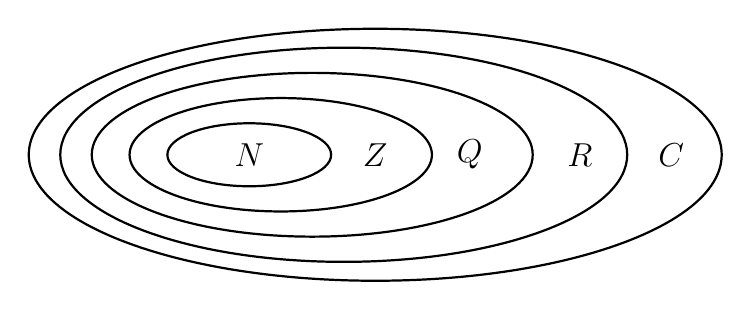
\begin{tikzpicture}[scale=.8, every node/.style={font=\large}]
  % Complex numbers (outermost)
  \draw[thick] (0,0) ellipse (5.5 and 2);
  \node at (4.7,0) {$\mathbb{C}$};

  % Real numbers
  \draw[thick] (-0.5,0) ellipse (4.5 and 1.7);
  \node at (3.25,0) {$\mathbb{R}$};

  % Rational numbers
  \draw[thick] (-1.0,0) ellipse (3.5 and 1.3);
  \node at (1.5,0) {$\mathbb{Q}$};

  % Integers
  \draw[thick] (-1.5,0) ellipse (2.4 and 0.9);
  \node at (0,0) {$\mathbb{Z}$};

  % Natural numbers
  \draw[thick] (-2.0,0) ellipse (1.3 and 0.5);
  \node at (-2,0) {$\mathbb{N}$};
\end{tikzpicture}
\captionof{figure}{Mengenbeziehungen der Zahlenmengen} 
\end{center}

\begin{bsp} Im Folgenden sind einige Zahlen für die jeweiligen Zahlenmengen angegeben \vspace{5pt}\\
rationale Zahlen: \(1,\,-2,\,\frac{4}{3}=1.\dot{3},\,\frac{5}{2}=2.5,\,\frac{1}{3}=0.\dot{3}\) \vspace{3pt}\\
irrationale Zahlen: \(\sqrt{2},\,\sqrt{3},\,e=2.71828...,\,\pi=3.1415...\) \vspace{3pt}\\
reelle Zahlen: \(-2,\,\frac{4}{3}=1.\dot{3},\,\frac{5}{2}=2.5,\,e,\,pi,\,\sqrt{3}\) \vspace{3pt}\\
komplexe Zahlen \(4+3\veci,\, 10\veci,\, 8-\veci\)
\end{bsp}

\subsubsection{Intervalle}
Abgeschlossene Intervalle werden mit eckigen Klammern geschrieben und beinhalten auch die beiden Randpunkte:
\begin{equation}
    [a,b] = \{x \in \R : a \leq x \leq b\}
\end{equation}
Bei offenen Intervallen werden runde Klammern verwendet. Die Randpunkte sind hier nicht enthalten:
\begin{equation}
    (a,b) = \{x \in \R : a < x < b\}
\end{equation}
Intervalle können auch auf einer Seite offen und auf der anderen Seite geschlossen sein. Kommt die Zahl $\infty$ vor so ist immer eine Klammer zu verwenden.
\begin{bsp}
    \begin{equation*}
        [5,\infty) = \{ x \in \R : x \geq 5 \}
    \end{equation*}
\end{bsp}
\subsubsection{Betrag einer Zahl}
Der Betrag einer Zahl (auch Absolutwert genannt) beschreibt, wie weit eine Zahl vom Nullpunkt entfernt ist (ohne Vorzeichen) und ist wie folgt definiert:
\begin{equation}
    |x| =
    \begin{cases}
        x, & \text{wenn } x \ge 0, \\
        -x, & \text{wenn } x < 0.
    \end{cases}
\end{equation}
Das bedeutet wenn \(x\) positiv oder 0 ist bleibt der Wert der Zahl gleich und wenn x negativ ist wird das Minuszeichen entfernt.

\subsection{(Un-)Gleichungen und Gleichungssysteme}
Verbindet man zwei Therme (linke und rechte Seite) durch ein Gleichheitszeichen, erhält man eine Gleichung. Diese Gleichung enthält eine Unbekannte, welche durch \textbf{Äquivalenzumformungen} berechnet werden kann. \\
Die \textbf{Grundmenge} \(G\) ist die Menge aller Zahlen, aus denen die Lösungen einer Gleichung stammen dürfen. Sie legt also fest, in welchem Zahlenbereich man arbeitet. \\
Die \textbf{Definitionsmenge} \(D\) umfasst die Zahlen die man in die Gleichung einsetzen darf:
\begin{itemize}
    \item keine Division durch 0
    \item keine Wurzeln aus negativen Zahlen
    \item kein Logarithmus von negativen Zahlen
\end{itemize}
Die \textbf{Lösungsmenge} \(L\) enthält alle Lösungen einer Gleichung und kann auch leer sein oder die ganze Definitionsmenge enthalten.
\begin{aufgabe}
    Gib die Defintionsmenge folgender Gleichungen an: \\
    \[
        \frac{1}{x}=2,\quad 2\cdot x+3=5,\quad \frac{5x-3}{x-1},\quad \sqrt{x+3}=5
    \]
\end{aufgabe}
\begin{loesung}
    \[
        D_1=\R \setminus \{0\}, \quad
        D_2=\R, \quad
        D_3=\R \setminus \{1\}, \quad
        D_4=[-3,\infty)
    \]
\end{loesung}
\subsubsection{Lineare Gleichungen}
Lineare Gleichungen sind Gleichungen in denen die Unbekannte nur in der ersten Potenz vorkommt:
\begin{equation}
    a \cdot x + b = 0,\quad a,b \in \R
\end{equation}
Ihre Lösung kann als Nullstelle der zugehörigen linearen Funktion \(f(x)=k\cdot x + d\) interpretiert werden.
\begin{aufgabe}
    Ermittle die Lösung folgender linearer Gleichung: \(2\cdot x - 3 = 0\)
\end{aufgabe}
\begin{loesung}
    \begin{align*}
        2\cdot x - 3 &= 0 \\
        2\cdot x &= 3 \\
        x &= \frac{3}{2} = 1.5
    \end{align*}
\end{loesung}
\begin{geogebracode}
Löse(2*x-3=0,x)   // Symbolische Lösung
NLöse(2*x-3=0,x)  // Numerische Lösung
\end{geogebracode}
\subsubsection{Lineare Ungleichungen}
Lineare Ungleichungen sind wie lineare Gleichungen, nur dass statt dem Gleichheitszeichen ein Ungleichheitszeichen verwendet wird.
\begin{equation}
    ax + b < c, \quad ax + b \le c, \quad ax + b > c, \quad ax + b \ge c
\end{equation}
Die Unbekannte kann wieder durch Äquivalenzumformungen bestimmt werden, jedoch muss man beim multiplizieren oder dividieren einer negativen Zahl das Ungleichheitszeichen umdrehen.
\begin{bsp}
    Löse folgende Ungleichung: \(-4x+8>0\)
    \begin{align*}        
        -4x+8&>0 \\
        -4x&>-8 \\
        4x&<8 \\
        x&<2
    \end{align*}
\end{bsp}
\noindent
Das Lösen von Ungleichungen wird oft zur Bestimmung der Definitionsmenge benötigt.
\begin{aufgabe}
    Bestimme die Definitionsmenge folgender Gleichung: \(\sqrt{-2x-3}=0\)
\end{aufgabe}
\begin{loesung}
\vspace{-12pt}
    \begin{align*}
        -2x-3&>0 \\
        -2x&>3 \\
        x&<-\frac{3}{2}
    \end{align*}
\end{loesung}
\begin{geogebracode}
    Löse(-2*x-3>0,x) // CAS
\end{geogebracode}
\subsubsection{Quadratische Gleichungen}
Lineare Gleichungen sind Gleichungen in denen die Unbekannte maximal in der zweiten Potenz vor-
kommt:
\[
    ax^2+bx+c=0
\]
Die Lösungen können als Nullstellen der zugehörigen quadratischen Funktion \(f(x)=ax^2+bx+c\) interpretiert werden.
Die Lösungen können entweder über die kleine Lösungsformel (\ref{eq:klLoes}) oder die große Lösungsformel (\ref{eq:grLoes}) berechnet werden.
\begin{equation}\label{eq:klLoes}
    x_{1,2} = -\frac{p}{2} \pm \sqrt{\left(\frac{p}{2}\right)^2 - q}
\end{equation}
\begin{equation}\label{eq:grLoes}
    x_{1,2} = \frac{-b \pm \sqrt{b^2 - 4ac}}{2a} 
\end{equation}
Bei den Lösungen von quadratischen Gleichungen muss man im Allgemeinen zwischen 3 Fällen unterscheiden. Hierfür definiert man zuerst die Diskriminante (Zahl unter der Wurzel):
\begin{equation}
    D = b^2 - 4ac.
\end{equation}
\begin{itemize}
    \item \textbf{Fall 1: $D > 0$}    es gibt zwei verschiedene reelle Lösungen
    \item \textbf{Fall 2: $D = 0$}    eine doppelte reelle Lösung da der Wurzelausdruck wegfällt
    \item \textbf{Fall 3: $D < 0$}    zwei komplexe Lösungen da die Wurzel einer negativen Zahl gezogen wird
\end{itemize}
Diese drei Fälle können auch sehr gut graphisch mit Parabeln dargestellt werden (2.2).
\begin{aufgabe}
    Berechne die Lösungen folgender Gleichung: \(2x^{2}+4x-6=0\)
\end{aufgabe}
\begin{loesung}
    \\Zuerst bestimmen wir: \(a=2,\;b=4,\;c=-6\) \\
    jetzt können wir die die große Lösungsformel (\ref{eq:grLoes}) verwenden:
    \begin{align*}
        x_{1,2} = \frac{-b \pm \sqrt{b^2 - 4ac}}{2a} &= \frac{-4 \pm \sqrt{4^2 - 4\cdot2\cdot(-6)}}{2\cdot2} \\
        x_{1,2} &= \frac{-4 \pm \sqrt{64}}{4} \\
        x_{1,2} &= \{-3,\;1\}
    \end{align*}
    wir haben zwei verschiedene reelle Lösungen was zu erwarten war da die Diskriminante größer als 0 ist.
    \[
        D=b^2-4ac=4^2 - 4\cdot2\cdot(-6)=64>0
    \]
    Alternativ kann die Gleichung auch auf die Form \(x^2+bx+c=0\) gebracht werden und mit der kleinen Lösungsformel (\ref{eq:klLoes}) berechnet werden.
\end{loesung}
\begin{geogebracode}
    Löse(2*x^2+4*x-6=0,x) // CAS
    NLöse(2*x^2+4*x-6=0,x) 
\end{geogebracode}
\pagebreak
\subsubsection{Lineare Gleichungssysteme}
Ein lineares Gleichungssystem mit zwei Variablen besteht aus zwei linearen Gleichungen in den Unbekannten \(x\) und \(y\). Gesucht sind diejenigen Wertepaare \((x,y)\), die beide Gleichungen gleichzeitig erfüllen.  
\begin{align}  
    \text{I:}\;  &a_1 x + b_1 y = c_1  \\
    \text{II:}\; &a_2 x + b_2 y = c_2  \nonumber
\end{align}  
In Matrixform sieht dieses System folgendermaßen aus:
\begin{equation}
    \begin{pmatrix}  
        a_1 & b_1 \\  
        a_2 & b_2  
    \end{pmatrix}  
    \begin{pmatrix}  
        x \\  
        y  
    \end{pmatrix}  
    =  
    \begin{pmatrix}  
        c_1 \\  
        c_2  
    \end{pmatrix}
\end{equation}

\vspace{1em}  

\noindent  
\begin{minipage}{0.5\textwidth}  
\textbf{Eindeutige Lösung}  
\begin{align*}
    \text{I:}\; &x + y = 4 \qquad (y=-x+4) \\
    \text{II:}\; &x - y = 2 \qquad (y=x-2) 
\end{align*}
Die Geraden schneiden sich an einem Punkt.
Lösung: \((x,y) = (3,1)\).  
\end{minipage}  
\hfill  
\begin{minipage}{0.45\textwidth}  
\centering  
\begin{tikzpicture}  
\begin{axis}[axis lines=middle, xmin=-1, xmax=5, ymin=-1, ymax=5, grid=both, minor tick num=1,         width=7cm, height=6cm,
 xlabel={$x$}, ylabel={$y$}]  
    \addplot[domain=-1:5, samples=100, accent2, very thick] {4 - x};  
    \node[above right, accent2] at (axis cs:0.7,3.2) {$x + y = 4$};  

    \addplot[domain=-1:5, samples=100, accent, very thick] {x - 2};  
    \node[above left, accent] at (axis cs:4,2) {$x - y = 2$};  
  
    \addplot[only marks, mark=*, mark size=2pt] coordinates {(3,1)};  
    \node[left=4pt] at (axis cs:3,1) {$(3,1)$};  
\end{axis}  
\end{tikzpicture}  
\end{minipage}  
\\
\vspace{2em}  
  
\noindent  
\begin{minipage}{0.5\textwidth}  
\textbf{Keine Lösung}  
\begin{align*}
    \text{I:}\; &x + y = 2 \qquad (y=-x+2)\\  
    \text{II:}\; &x + y = 4 \qquad (y=-x+4)
\end{align*}
Die Geraden sind parallel und schneiden sich nicht. Dies ist der Fall, wenn die linken Seiten ein Vielfaches voneinander sind, die rechten nicht. Es gibt es keine gemeinsame Lösung.  
\end{minipage}  
\hfill  
\begin{minipage}{0.45\textwidth}  
\centering  
\begin{tikzpicture}  
\begin{axis}[axis lines=middle, xmin=-1, xmax=5, ymin=-1, ymax=5, grid=both, minor tick num=1, width=7cm, height=6cm, xlabel={$x$}, ylabel={$y$}]  
    % (I) x + y = 2  ->  y = 2 - x  
    \addplot[domain=-1:5, samples=100, accent2, very thick] {2 - x};  
    \node[below left, accent2] at (axis cs:1.2,1) {$x + y = 2$};  
  
    % (II) x + y = 4  ->  y = 4 - x  
    \addplot[domain=-1:5, samples=100, accent, very thick] {4 - x};  
    \node[above right, accent] at (axis cs:0.7,3.2) {$x + y = 4$};  
\end{axis}  
\end{tikzpicture}  
\end{minipage}  
\\
\vspace{2em}  
  
\noindent  
\begin{minipage}{0.5\textwidth}  
\textbf{Unendlich viele Lösungen}  
\begin{align*}  
    \text{I:}\; x + 2y = 4    \qquad (y=-x/2+2) \\  
    \text{II:}\; 2x + 4y = 8  \qquad (y=-x/2+2)
\end{align*}  
Die zweite Gleichung ist ein Vielfaches der ersten, also beschreiben beide dieselbe Gerade; jedes Punktpaar auf der Geraden ist Lösung.  
\end{minipage}  
\hfill  
\begin{minipage}{0.45\textwidth}  
\centering
\begin{tikzpicture}  
\begin{axis}[axis lines=middle, xmin=-1, xmax=5, ymin=-1, ymax=5, grid=both, minor tick num=1, width=7cm, height=6cm, xlabel={$x$}, ylabel={$y$}]  
    \addplot[domain=-1:5, samples=100, accent, very thick] {(4 - x)/2};  
    \node[above right, accent2] at (axis cs:0,2) {$x + 2y = 4$};  
  
    %\addplot[domain=-1:5, samples=100, purple, dashed, very thick] {(4 - x)/2};  
    \node[above right, accent] at (axis cs:2,1) {$2x + 4y = 8$};  
\end{axis}  
\end{tikzpicture}  
\end{minipage}
\\
\bigskip
\begin{geogebracode}
    g1: x+y=4 
    g2: x-y=2
    Löse({g1,g2},{x,y})
\end{geogebracode}


\pagebreak
\subsection{Vektoren}
Ein \textbf{Vektor} ist ein geometrisches Objekt, das sowohl eine \textit{Richtung} als auch eine \textit{Länge} besitzt. Ein Vektor wird meist als Spaltenmatrix dargestellt:
\begin{equation}
\vec{a} = 
\begin{pmatrix}
a_1 \\ a_2
\end{pmatrix} \in \mathbb{R}^2, \quad
\vec{b} = 
\begin{pmatrix}
b_1 \\ b_2 \\ b_3
\end{pmatrix} \in \mathbb{R}^3
\end{equation}
\noindent
Im 2D- oder 3D-Raum wird ein Vektor durch einen Pfeil dargestellt, dessen Länge der Betrag des Vektors ist und dessen Richtung die Orientierung angibt.
Möchte man einen Vektor eine genaue Position geben, braucht man einen Startpunkt von dem der Vektor ausgehen soll. Weiters kann man auch einen Vektor zwischen zwei Punkten definieren.

\begin{center}
\begin{tikzpicture}[scale=1.2, >=stealth]
    \draw[dashed, thick, black] (0,0) -- (2,0) node[midway, below] {$a_x$};
    \draw[dashed, thick, black] (2,0) -- (2,1) node[midway, right] {$a_y$};
    \draw[->, ultra thick, accent] (0,0) -- (2,1) node[midway, above] {$\vec{a}$};
    \fill (0,0) circle (1.5pt) node[left] {$P$};
    
    \fill (6.5,1) circle (1.5pt) node[above=2pt] {$B$};
    \draw[->, ultra thick, accent] (4,0) -- (6.5,1) node[midway, above=2pt] {$\vec{AB}$};
    \fill (4,0) circle (1.5pt) node[above=2pt] {$A$};
    
    \draw[->, thick] (-1,-.5) -- (7,-.5) node[right] {$x$};
    \draw[->, thick] (3,-1) -- (3,1.5) node[above] {$y$};
\end{tikzpicture}
\captionof{figure}{Graphische Darstellung eines zweidimensionalen Vektors $\vec{a}$ und einem Vektor zwischen zwei Punkten $\vec{AB}$}
\end{center}

\subsubsection{Addition/Subtraktion von Vektoren}
Die Addition/Subtraktion von Vektoren erfolgt komponentenweise:
\begin{equation}
\vec{u} \pm \vec{v} = 
\begin{pmatrix} a_1 \\ a_2 \\ a_3 \end{pmatrix} \pm
\begin{pmatrix} b_1 \\ b_2 \\ b_3 \end{pmatrix} =
\begin{pmatrix} a_1 \pm b_1 \\ a_2 \pm b_2 \\ a_3 \pm b_3\end{pmatrix}
\end{equation}
\noindent
\begin{minipage}[c]{0.6\textwidth}
Bei der graphischen \textbf{Vektoraddition} wird an die Spitze des Vektors $\vec{a}$ der Vektor $\vec{b}$ angesetzt. Verbindet man nun den Schaft von $\vec{a}$ mit der Spitze von $\vec{b}$ erhält man den Vektor $\vec{a+b}$. \\
Bei der graphischen \textbf{Vektorsubtraktion} geht man grundsätzlich wie bei der Addition vor. Man muss nur den Vektor $\vec{b}$ umkehren bzw. um 180° drehen.
\end{minipage}
\hspace{0.05\textwidth}
\begin{minipage}[c]{0.35\textwidth}
\begin{tikzpicture}[scale=1, >=stealth]
  \draw[->,thick] (-0.5,0) -- (4,0) node[right] {$x$};
  \draw[->,thick] (0,-0.5) -- (0,3) node[above] {$y$};

  \draw[->, ultra thick, black] (0,0) -- (2.5,1.5) node[midway, above] {$\vec{a}$};
  \draw[->, ultra thick, black] (2.5,1.5) -- (1.5,2.5) node[midway, above right] {$\vec{b}$};
  \draw[->, ultra thick, black, dashed] (2.5,1.5) -- (3.5,0.5) node[midway, above right] {$-\vec{b}$};
  \draw[->, ultra thick, accent] (0,0) -- (1.5,2.5) node[pos=.7, above left] {$\vec{a}+\vec{b}$};
  \draw[->, ultra thick, accent] (0,0) -- (3.5,0.5) node[pos=.7, above] {$\vec{a}-\vec{b}$};
\end{tikzpicture}
\end{minipage}

\subsubsection{Vektor zwischen zwei Punkten}
Der Verbindungsvektor zwischen zwei Punkten ist wie folgt definiert:
\begin{equation}
    \vv{AB} = \vv{B} - \vv{A} = 
    \begin{pmatrix} B_x-A_x \\ B_y-A_y \\ B_z-A_z \end{pmatrix}
\end{equation}

\subsubsection{Multiplikation mit einem Skalar}
Die Multiplikation eines Vektors mit einem Skalar erfolgt wieder komponentenweise:
\begin{equation}
s \vec{a} =
s
\begin{pmatrix} a_1 \\ a_2 \\ a_3 \end{pmatrix} =
\begin{pmatrix} s a_1 \\ s a_2 \\ s a_3 \end{pmatrix}, \quad s \in \mathbb{R}
\end{equation}
Graphisch kann die skalare Multiplikation als eine Streckung (\(s>1\)) oder Stauchung (\(0<s<1\)) bzw. eine Umkehrung (\(s<0\)) gesehen werden.
\subsubsection{Betrag eines Vektors}
Der Betrag bzw. die Norm eines Vektors ergibt die Länge des Pfeils und ist wie folgt definiert:
\begin{equation}
\|\vec{a}\| = \sqrt{a_1^2 + a_2^2 + a_3^2}
\end{equation}
\subsubsection{Einheitsvektor}
Wenn man einen Vektor durch seinen Betrag (=Länge) dividiert bekommt man den zugehörigen Einheitsvektor:
\begin{equation}
    \vec{a}_0 = \frac{1}{|a|}\vec{a}
\end{equation}
Der Einheitsvektor \(\vec{a}_0\) hat die gleiche Orientierung wie \(\vec{a}\) und einen Betrag von 1.
\subsubsection{Skalarprodukt}
Das Skalarprodukt ist eine Rechenoperation zwischen zwei Vektoren, die eine Zahl (Skalar) als Ergebnis liefert.
\begin{align}
    \vec{a} \cdot \vec{b} = a_1 b_1 + a_2 b_2 \\
    \vec{a} \cdot \vec{b} = a_1 b_1 + a_2 b_2  + a_3 b_3 
\end{align}
Alternativ kann das Skalarprodukt auch über den Winkel zwischen den beiden Vektoren berechnet werden:
\begin{equation}
    \vec{a}\cdot\vec{b} = |\vec{a}|\cdot|\vec{b}|\cdot\cos{(\alpha)}
\end{equation}
Durch Umformen erhält man die Formel für den Winkel zwischen zwei Vektoren:
\begin{equation}
    \alpha = \arccos{\left(\frac{\vec{a}\cdot\vec{b}}{|\vec{a}|\cdot|\vec{b}|}\right)}
\end{equation}
Eine wichtige Eigenschaft des Skalarproduktes ist auch das es 0 ergibt sobald zwei Vektoren senkrecht/im rechten Winkel zueinander stehen (\(\vec{a}\perp \vec{b}\)). Man sagt hier auch dass die Vektoren orthogonal sind.\\
Mit dieser Information kann man auch die Formel für Normalvektoren herleiten:
\begin{equation}
    \vec{a} = \begin{pmatrix} a_1 \\ a_2 \end{pmatrix},\quad 
    \vec{n} = \begin{pmatrix} n_1 \\ n_2 \end{pmatrix},
\end{equation}
Um Orthogonalität zu verlangen setzt man das Skalarprodukt 0:
\begin{equation}
    \vec{a} \cdot \vec{n} = a_1 n_1 + a_2 n_2 = a_1\cdot(-a_2) + a_2\cdot a_1=0
\end{equation}
Hierbei kann man erkennen, dass diese Bedingung durch Vertauschen beider Koordinaten und eines Vorzeichens erfüllt wird. Man erhält schließlich die Formel für alle Normalvektoren:
\begin{equation}
    \vec{n} = s\cdot\begin{pmatrix} -a_2 \\ a_1 \end{pmatrix}
\end{equation}

\subsubsection{Vektorprodukt (Kreuzprodukt)}
Das Kreuzprodukt ist eine Operation für zwei Vektoren im dreidimensionalen Raum und ist wie folgt definiert:
\begin{equation}
\vec{a} \times \vec{b} = 
\begin{pmatrix}
a_2 b_3 - a_3 b_2 \\
a_3 b_1 - a_1 b_3 \\
a_1 b_2 - a_2 b_1
\end{pmatrix}
\end{equation}
Das Ergebnis des Kreuzproduktes ist wieder ein Vektor, welcher orthogonal auf beide Vektoren steht. Der Betrag (=Länge) dieses Vektors entspricht genau der Fläche des aufgespannten Parallelogramms. \\
\begin{center}
\begin{tikzpicture}
\draw[-,thick,fill=white!95!red](0,0)--(3,0)--(4,1)--(1,1)--cycle;
\node at (2,0.5) {$|{a}\times {b}|$};
\draw[ultra thick,-latex,black](0,0)--(3,0)node[midway,below]{$a$};
\draw[ultra thick,-latex,black](0,0)--(1,1)node[midway,above]{$b$};
\draw[ultra thick,-latex,accent](0,0)--(0,3)node[pos=0.7,right]{$a\times b$};
\draw[thick] (0.6,0) arc [start angle=0,end angle=45,radius=0.6]
node[pos=0.7,right]{$\alpha$};
\end{tikzpicture}
%\captionof{figure}{Graphische Bedeutung des Kreuzproduktes}
\end{center}

\subsubsection{Parameterdarstellung einer Geraden}
Die Parameterdarstellung ist eine Möglichkeit, eine Gerade im zwei- oder dreidimensionalen Raum darzustellen.
\begin{equation}
    g:\;X=P+t\vec{g}
\end{equation}
Der Punkt $X$ stellt alle Punkte auf der Geraden dar. Ausgehend von Stützpunk $P$ kann man durch das Skalieren des Richtungsvektors $\vec{g}$ alle Punkte auf der Geraden erreichen.

\begin{center}
\begin{tikzpicture}[scale=1, >=stealth]
    \draw[->,thick] (-0.5,0) -- (3,0) node[right] {$x$};
    \draw[->,thick] (0,-0.5) -- (0,2.5) node[above] {$y$};
    \draw[-, ultra thick, black] (-.5,-3/8) -- (3,9/4) node[pos=.9, below] {$g$};
    \draw[->, ultra thick, accent] (1,3/4) -- (2,1.5) node[midway, above left] {$\vec{g}$};
    \fill (1,3/4) circle (1.5pt) node[below] {$P$};
\end{tikzpicture}
\captionof{figure}{Paramterdarstellung einer Geraden im $\R^2$}
\end{center}

\subsubsection{Normalvektordarstellung}
Die Normalvektordarstellung beschreibt eine Gerade über einen Vektor $\vec{n}$, der senkrecht zu der Geraden steht.
\begin{equation}
    g:\;\vec{n}\cdot X=\vec{n}\cdot P
\end{equation}
Dabei ist $P$ ein Punkt auf der Geraden (Stützpunkt) und $X$ ein beliebiger Punkt auf der Geraden.  
\begin{center}
\begin{tikzpicture}[scale=1, >=stealth]
    \draw[->,thick] (-0.5,0) -- (3,0) node[right] {$x$};
    \draw[->,thick] (0,-0.5) -- (0,2.5) node[above] {$y$};
    \draw[-, ultra thick, black] (-.5,-3/8) -- (3,9/4) node[pos=.9, below] {$g$};
    \draw[->, ultra thick, accent] (1,3/4) -- ++(-3/4,1) node[midway, above right] {$\vec{n}$};
    \fill (1,3/4) circle (1.5pt) node[below] {$P$};
\end{tikzpicture}
\captionof{figure}{Normalvektordarstellung einer Geraden im $\R^2$}
\end{center}

\subsubsection{Hauptform}
Die Hauptform ist eine Koordinatenschreibweise der Normalvektordarstellung.
\begin{equation}
    g:\;a x + b y = c
\end{equation}
Einen Normalvektor und Richtungsvektor kann man direkt ablesen.
\begin{equation}
    \vec{n}=\begin{pmatrix} a \\ b \end{pmatrix},\quad 
    \vec{g} = \begin{pmatrix} -b \\ a \end{pmatrix}
\end{equation}
Formt man die Hauptform etwas um, so erhält man die bereits bekannte Form einer linearen Funktion ($y = k x + d$).
\begin{align}
    a x + b y = c \\
    b y = -a x + c \\
    y = -\frac{a}{b} x + \frac{c}{b}
\end{align}

\subsubsection{Aufgaben zu Vektoren}
\begin{aufgabe}
Gegeben sind die Punkte \(A=(1,2),\;B=(3,5),\;C=(3,3),\;D=(1,4)\)
    \begin{itemize}
        \item[1.] Berechne die Verbindungsvektoren \(\vv{AB}\) und \(\vv{CD}\)
        \item[2.] Berechne das Skalarprodukt \(\vv{AB} \cdot \vv{CD}\)
        \item[3.] Berechne die Länge der Pfeile \(\vv{AB}\) und \(\vv{CD}\)
        \item[4.] Gib einen Normalvektor \(\vec{n}\) zu \(\vv{AB}\) an
        \item[5.] Berechne den Einheitsvektor \(\vv{AB}_0\)
        \item[6.] Die Gerade $g$ verläuft durch die Punkte $A$ und $B$. Überprüfe ob die Punkte \(E(5,8)\) und \(F=(2,3)\) auf der Geraden $g$ liegen.
        \item[7.] Gib die Gerade in Normalvektorform und Hauptform an
    \end{itemize}
\end{aufgabe}
\begin{loesung}
    \begin{itemize}
        \item[1.] Verbindungsvektoren:
        \[
            \vv{AB} = B - A = 
            \begin{pmatrix}3 \\ 5\end{pmatrix} -
            \begin{pmatrix}1 \\ 2\end{pmatrix} =
            \begin{pmatrix}2 \\ 3\end{pmatrix}, \qquad
            \vv{CD} = D - C =
            \begin{pmatrix}1 \\ 4\end{pmatrix} -
            \begin{pmatrix}3 \\ 3\end{pmatrix} =
            \begin{pmatrix}-2 \\ 1\end{pmatrix}.
        \]
        \item[2.] Skalarprodukt:
        \[
            \vv{AB} \cdot \vv{CD} =
            \begin{pmatrix}2 \\ 3\end{pmatrix} \cdot
            \begin{pmatrix}-2 \\ 1\end{pmatrix}
            = 2 \cdot (-2) + 3 \cdot 1
            = -4 + 3 = -1.
        \]
        \item[3.] Längen der Vektoren:
        \[
            \|\vv{AB}\| = \sqrt{2^2 + 3^2} = \sqrt{4 + 9} = \sqrt{13},
            \qquad
            \|\vv{CD}\| = \sqrt{(-2)^2 + 1^2} = \sqrt{4 + 1} = \sqrt{5}.
        \]
        \item[4.] Normalvektor zu \(\vv{AB}\): \\
        Wir vertauschen $x$ und $y$ Koordinate und ändern ein Vorzeichen:
        \[
            \vec{n} = \begin{pmatrix}-3 \\ 2\end{pmatrix}
        \]
        \item[5.] Einheitsvektor \(\vv{AB}_0\):
        \[
            \vv{AB}_0 = \frac{1}{\|\vv{AB}\|} \vv{AB}
            = \frac{1}{\sqrt{13}}
            \begin{pmatrix}2 \\ 3\end{pmatrix}
            =
            \begin{pmatrix}\dfrac{2}{\sqrt{13}} \\[4pt] \dfrac{3}{\sqrt{13}}\end{pmatrix}.
        \]
    
        \item[6.] Überprüfen, ob \(E\) und \(F\) auf der Geraden \(g\) durch \(A\) und \(B\) liegen.
        Eine Parametergleichung von \(g\) lautet:
        \begin{align*}
            g:\;\; X &= P + t \cdot \vec{g} \\
            g:\;\; X &= \begin{pmatrix}1 \\ 2\end{pmatrix} + t \begin{pmatrix}2 \\ 3\end{pmatrix}
        \end{align*}
        Punkt \(E(5,8)\):
        Wir suchen ein \(t\) mit
        \[
            \begin{pmatrix}5 \\ 8\end{pmatrix} =
            \begin{pmatrix}1 \\ 2\end{pmatrix}
            + t \begin{pmatrix}2 \\ 3\end{pmatrix}      
            \;\Rightarrow\;
            \begin{cases}
                1 + 2t = 5, \\
                2 + 3t = 8.
            \end{cases}
        \]
        Beide Gleichungen liefern dasselbe \(t=2\), also liegt \(E\) auf \(g\).
        Punkt \(F(2,3)\):
        \[
            \begin{pmatrix}2 \\ 3\end{pmatrix} =
            \begin{pmatrix}1 \\ 2\end{pmatrix}
            + t \begin{pmatrix}2 \\ 3\end{pmatrix}
            \;\Rightarrow\;
            \begin{cases}
                1 + 2t = 2, \\
                2 + 3t = 3.
            \end{cases}
        \]
        Die erste Gleichung liefert $t=\frac{1}{2}$ und die zweite Gleichung $t=\frac{1}{3}$. Es gibt kein gemeinsames \(t\), also liegt \(F\) \emph{nicht} auf der Geraden \(g\).

        \item[7.] Um die Normalvektorform zu finden können wir den Richtungsvektor $\vec{g}$ um $90^\circ$ rotieren:
        \[
            \vec{n} = \begin{pmatrix} -3 \\ 2 \end{pmatrix}
        \]
        Als Stützpunkt können wir $P$ beibehalten und erhalten als Lösung: 
        \[
            \vec{n} \cdot X = \vec{n} \cdot P
        \]
        \[
            \begin{pmatrix} -3 \\ 2 \end{pmatrix} \cdot X = 
            \begin{pmatrix} -3 \\ 2 \end{pmatrix} \cdot 
            \begin{pmatrix}  1 \\ 2 \end{pmatrix} 
        \]
        Die Hauptform erhalten wir indem wir die Skalarprodukte in der Normalvektorform berechnen.
        \[
            -3x + 2y = -3 \cdot 1 + 2 \cdot 2
        \]
        \[
            -3x + 2y = 1
        \]
    \end{itemize}
\end{loesung}

\begin{geogebracode}
    // Punkte definieren
    A=(1,2)
    B=(3,5)
    C=(3,3)
    D=(1,4)

    // Vektoren aus den Punkten Konstruieren
    AB=Vektor(A,B)
    CD=Vektor(C,D)

    // Berechnungen durchführen
    Skalarprodukt(AB,CD)
    Länge(AB)
    Länge(CD)
    Normalvektor(AB)
    Einheitsvektor(AB)

    // Geradengleichung definieren
    X = A + t*AB

    // Punkte E und F definieren
    E=(5,8)
    F=(2,3)

    // Überprüfen ob die 3 Punkte auf einer Geraden liegen
    LiegenAufGerade(A, B, E)
    LiegenAufGerade(A, B, F)
\end{geogebracode}

\pagebreak
\subsection{Trigonometrie}
\subsubsection{Grundlagen}

\begin{minipage}{0.4\textwidth}
\textbf{Umfang und Flächeninhalt}
\begin{equation}
    U=a+b+c
\end{equation}
\begin{equation}
    A=\frac{a\cdot h_a}{2}=\frac{b\cdot h_b}{2}=\frac{c\cdot h_c}{2}
\end{equation}
\end{minipage}
\hspace{0.1\textwidth}
\begin{minipage}{0.5\textwidth}
\begin{tikzpicture}[scale=.7, >=stealth]
  \draw[thick] (0,0) coordinate[label=below left:$A$] (A) --node[midway,below]{c}
        (6,0) coordinate[label=below right:$B$] (B) --node[midway,above right]{a}
        (4,4) coordinate[label=above:$C$] (C) --node[midway,above left]{b}
        cycle;

    \draw[-, thick, accent] (4,0) -- (4,4) node[pos=0.3, below right] {$h_c$};
    \draw[-, thick, accent] (3,3) -- (6,0) node[midway, right] {$h_b$};
    \draw[-, thick, accent] (4.8,2.4) -- (0,0) node[midway, below] {$h_a$};
\end{tikzpicture}
\end{minipage}
\\
\textbf{Winkelbeziehungen}\\
\noindent
\begin{minipage}[t]{.33\textwidth}
\begin{center}
\begin{tikzpicture}
\draw[line width=.4mm] (13,0) coordinate (A) --node[midway,below]{}
        (15.5,0) coordinate (B) --node[midway,above right]{}
        (14.5,1.5) coordinate (C) --node[midway,above left]{}
        cycle;
\pic[pic text=$\alpha$,accent,thick,draw,angle radius=.8cm] {angle=B--A--C};
\pic[pic text=$\beta$,accent,thick,draw,angle radius=.8cm] {angle=C--B--A};
\pic[pic text=$\gamma$,accent,thick,draw,angle radius=.7cm] {angle=A--C--B};
\end{tikzpicture}
\captionof*{figure}{$\alpha+\beta+\gamma=180^\circ$}
\end{center}
\end{minipage}
\begin{minipage}[t]{.33\textwidth}
\begin{center}
\begin{tikzpicture}[scale=1.0, >=stealth]
    \draw [line width=.4mm]
        (3,0) coordinate (A) -- 
        (1.5,0) coordinate (B) --
        (2.8,1.3) coordinate (C)
        pic [pic text=$\alpha$, draw=accent,->, angle radius=.8cm] {angle};
    \draw [line width=.4mm]
        (2.8,1.3) coordinate (A)
        (1.5,0) coordinate (B) --
        (0,0) coordinate (C)
        pic [pic text=$\beta$, draw=black,->, angle radius=.8cm] {angle};
    \draw [line width=.4mm]
        (0,0) coordinate (A)
        (1.5,0) coordinate (B) --
        (0.2,-1.3) coordinate (C)
        pic [pic text=$\alpha$, draw=accent,->, angle radius=.8cm] {angle};
    \draw [line width=.4mm]
        (0.2,-1.3) coordinate (A)
        (1.5,0) coordinate (B)
        (3,0) coordinate (C)
        pic [pic text=$\beta$, draw=black,->, angle radius=.8cm] {angle};
\end{tikzpicture}
\captionof*{figure}{$\alpha+\beta=180^\circ$}
\end{center}
\end{minipage}
\begin{minipage}[t]{.33\textwidth}
\begin{center}
\begin{tikzpicture}
\draw [line width=.4mm]
    (12.5,2) coordinate (A) --
    (9.5,2) coordinate (B) 
    (12,3) coordinate (C)
    pic [pic text=$\alpha/2$, draw=black,-, angle radius=1.8cm] {angle};
\draw [line width=.4mm]
    (12.5,2) coordinate (C) 
    (9.5,2) coordinate (B) 
    (12,1) coordinate (A)
    pic [pic text=$\alpha/2$, draw=black,-, angle radius=1.8cm] {angle};
\draw [line width=.4mm]
    (12,1) coordinate (A) --
    (9.5,2) coordinate (B) --
    (12,3) coordinate (C)
    pic [draw=accent,->, angle radius=2.3cm] {angle};
\end{tikzpicture}
\captionof*{figure}{$\frac{\alpha}{2}+\frac{\alpha}{2}=\alpha$}
\end{center}
\end{minipage}
\vspace{15pt}
\\
\noindent
\begin{minipage}[t]{.33\textwidth}
\begin{center}
\begin{tikzpicture}[scale=1.0, >=stealth]
    \draw [line width=.4mm]
        (2,0) coordinate (A) 
        (0,0) coordinate (B) --
        (1.4,1.4) coordinate (C)
    pic [pic text=$\alpha$, draw=black,-, angle radius=.9cm] {angle};
    \draw [line width=.4mm]
        (1.4,1.4) coordinate (A) 
        (0,0) coordinate (B) 
        (0,2) coordinate (C)
        pic [pic text=$\beta$, draw=black,-, angle radius=.9cm] {angle};
    \draw [line width=.4mm]
        (2,0) coordinate (A) -- 
        (0,0) coordinate (B) --
        (0,2) coordinate (C)
        pic [draw=accent,->, angle radius=1.4cm] {angle};
\end{tikzpicture}
\captionof*{figure}{$\alpha+\beta=90^\circ$}
\end{center}
\end{minipage}
\begin{minipage}[t]{.33\textwidth}
\begin{center}
\begin{tikzpicture}[scale=1.0, >=stealth]
    \draw [line width=.4mm]
        (3,0) coordinate (A) -- 
        (1.5,0) coordinate (B) --
        (0,0) coordinate (C)
        pic [draw=accent,->, angle radius=1.3cm] {angle};
    \draw [line width=.4mm]
        (3,0) coordinate (A) -- 
        (1.5,0) coordinate (B) --
        (2.8,1.3) coordinate (C)
        pic [pic text=$\gamma$, draw=black,-, angle radius=.9cm] {angle};
    \draw [line width=.4mm]
        (2.8,1.3) coordinate (A) -- 
        (1.5,0) coordinate (B) --
        (0.2,1.3) coordinate (C)
        pic [pic text=$\beta$, draw=black,-, angle radius=.9cm] {angle};
    \draw [line width=.4mm]
        (0.2,1.3) coordinate (A)
        (1.5,0) coordinate (B) --
        (0,0) coordinate (C)
        pic [pic text=$\alpha$, draw=black,-, angle radius=.9cm] {angle};
\end{tikzpicture}
\captionof*{figure}{$\alpha+\beta+\gamma=180^\circ$}
\end{center}
\end{minipage}
\begin{minipage}[t]{.33\textwidth}
\begin{center}
\begin{tikzpicture}
\draw [line width=.4mm]
    (1.7,1) coordinate (A) --
    (0,0) coordinate (B)
    (1,1.7) coordinate (C)
    pic [pic text=$\alpha$, draw=black,-, angle radius=1.1cm] {angle};
\draw [line width=.4mm]
    (2,0) coordinate (A) 
    (0,0) coordinate (B) 
    (1.7,1) coordinate (C)
    pic [pic text=$\beta$, draw=black,-, angle radius=1.1cm] {angle};
\draw [line width=.4mm]
    (2,0) coordinate (A) -- 
    (0,0) coordinate (B) --
    (1,1.7) coordinate (C)
    pic [draw=accent,->, angle radius=1.4cm] {angle};
\end{tikzpicture}
\captionof*{figure}{$\alpha+\beta=\gamma$}
\end{center}
\end{minipage}

\subsubsection{Grad- und Bogenmaß}
Gradmaß und Bogemaß sind zwei Möglichkeiten einen Winkel darzustellen. Eine vollständige Drehung entspricht $360^\circ$ (Grad) bzw. $2\pi$ rad (Radianten).
Die Umrechnung erfolgt über den Faktor $\pi/180$:
\begin{equation}
\theta_{\mathrm{rad}} = \theta_{\circ} \cdot \frac{\pi}{180^\circ}
\end{equation}
\begin{equation}
\theta_{\circ} = \theta_{\mathrm{rad}} \cdot \frac{180^\circ}{\pi}
\end{equation}

\subsubsection{Trigonometrie im allgemeinen Dreieck}
\begin{minipage}{0.4\textwidth}
\textbf{Sinussatz}
\begin{equation}
\frac{a}{\sin(\alpha)} = \frac{b}{\sin(\beta)} = \frac{c}{\sin(\gamma)}
\end{equation}
\textbf{Cosinussatz}
\begin{equation}
a^2 = b^2 + c^2 - 2bc \cdot \cos(\alpha)
\end{equation}
\begin{equation}
b^2 = a^2 + c^2 - 2ac \cdot \cos(\beta)
\end{equation}
\begin{equation}
c^2 = a^2 + b^2 - 2ab \cdot \cos(\gamma)
\end{equation}
\end{minipage}
\hspace{0.1\textwidth}
\begin{minipage}{0.5\textwidth}
\begin{tikzpicture}[scale=.9, >=stealth]
  \draw[thick] (0,0) coordinate[label=below left:$A$] (A) --node[midway,below]{c}
        (6,0) coordinate[label=below right:$B$] (B) --node[midway,above right]{a}
        (4,4) coordinate[label=above:$C$] (C) --node[midway,above left]{b}
        cycle;
        \pic[pic text=$\alpha$,accent,thick,draw,angle radius=1cm] {angle=B--A--C};
        \pic[pic text=$\beta$,accent,thick,draw,angle radius=1cm] {angle=C--B--A};
        \pic[pic text=$\gamma$,accent,thick,draw,angle radius=1cm] {angle=A--C--B};
\end{tikzpicture}
\end{minipage}
\\


\subsubsection{Trigonometrie im rechtwinkeligen Dreieck}
\begin{minipage}{0.5\textwidth}
\textbf{Satz des Pythagoras}
\begin{equation}
\begin{array}{c@{\;}c@{\;}c@{\;}c@{\;}c}
\mathrm{Kathete}^2 & + & \mathrm{Kathete}^2 & = & \mathrm{Hypotenuse}^2 \\[4pt]
a^2                & + & b^2                & = & c^2
\end{array}
\end{equation}


\textbf{Winkelbziehungen}
\begin{align}
    \sin{(\alpha)} &= \frac{\mathrm{Gegenkathete}}{\mathrm{Hypotenuse}} = \frac{b}{c} \\
    \cos{(\alpha)} &= \frac{\mathrm{Ankathete}}{\mathrm{Hypotenuse}} = \frac{a}{c} \\
    \tan{(\alpha)} &= \frac{\mathrm{Gegenkathete}}{\mathrm{Ankathete}} = \frac{b}{a}
\end{align}

\end{minipage}
\hspace{0.1\textwidth}
\begin{minipage}{0.4\textwidth}
\begin{tikzpicture}[scale=.9, >=stealth]
  \draw[thick] (0,0) coordinate[] (A) --node[midway,below, sloped]
        {\begin{tabular}{c} Ankathete von $\alpha$ \\ \textcolor{accent}{a} \end{tabular}}
        (6,0) coordinate[] (B) --node[midway, below, sloped]
        {\begin{tabular}{c} Gegenkathete von $\alpha$ \\ \textcolor{accent}{b} \end{tabular}}
        (6,4) coordinate[] (C) --node[midway, sloped, above]
        {\begin{tabular}{c} \textcolor{accent}{c} \\ Hypotenuse \end{tabular}}
        cycle;
        \pic[pic text=$\alpha$,accent,thick,draw,angle radius=1.5cm] {angle=B--A--C};
        \pic[pic text=$90^\circ$,black,thick,draw,angle radius=1cm] {angle=C--B--A};
\end{tikzpicture}
\end{minipage}
\vspace{12pt}
\\
\subsubsection{Umkehrfunktionen}
Um aus den Seitenverhältnissen die zughörigen Winkel zu berechnen, benötigt man die entsprechenden Umkehrfunktionen:
\begin{align}
    x_1 = \sin{(\alpha)},\quad \alpha = \arcsin{(x_1)} \\
    x_2 = \cos{(\beta)},\quad \beta = \arccos{(x_2)} \\
    x_3 = \tan{(\gamma)},\quad \gamma = \arctan{(x_3)} 
\end{align}

\noindent
\subsubsection{Steigungswinkel}
\begin{minipage}[c]{0.6\textwidth}
\begin{align}
    &\tan{(\alpha)} = \frac{\mathrm{Gegenkathete}}{\mathrm{Ankathete}} = \frac{\Delta y}{\Delta x} = k \\[1em]
    &\alpha = \arctan{\left(\frac{\mathrm{Gegenkathete}}{\mathrm{Ankathete}}\right)} = \arctan{\left(\frac{\Delta y}{\Delta x}\right)}
\end{align}
\\
\end{minipage}
\hspace{0.1\textwidth}
\begin{minipage}[]{0.3\textwidth}
\begin{tikzpicture}[scale=.7, >=stealth]
  \draw[thick] (0,0) coordinate[] (A) --node[midway,below, sloped]
        {\begin{tabular}{c} Ankathete \\ \textcolor{accent}{$\Delta$x} \end{tabular}}
        (6,0) coordinate[] (B) --node[midway, below, sloped]
        {\begin{tabular}{c} Gegenkathete \\ \textcolor{accent}{$\Delta$y} \end{tabular}}
        (6,4) coordinate[] (C) --node[midway, sloped, above]
        {Hypotenuse}
        cycle;
        \pic[pic text=$\alpha$,accent,thick,draw,angle radius=1.5cm] {angle=B--A--C};
        \pic[pic text=$90^\circ$,black,thick,draw,angle radius=1cm] {angle=C--B--A};
\end{tikzpicture}
\end{minipage}

\subsubsection{Strahlensatz}
\begin{minipage}[c]{0.3\textwidth}
\begin{equation}
    \frac{a}{a_1} = \frac{b}{b_1} = \frac{c}{c_1}
\end{equation}
\begin{equation}
    \frac{a_1}{a} = \frac{b_1}{b} = \frac{c_1}{c}
\end{equation}
\\
\end{minipage}
\hspace{0.1\textwidth}
\begin{minipage}[]{0.5\textwidth}
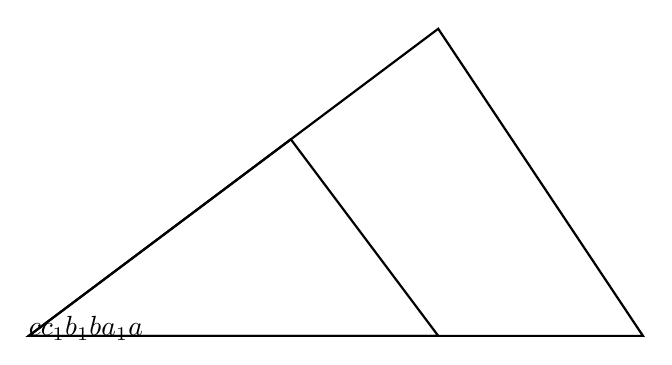
\begin{tikzpicture}[scale=1.3]

% First triangle
\draw[thick] (0,0) -- (6,0) -- (4,3) -- cycle;
\draw[thick] (0,0) -- (4,0) -- (2.56,1.92) -- cycle;

\dimline[line style={line width=0.7},color=black,extension start length=-0.05, extension end length=-0.05]
{(0,-.25)}{(4,-.25)}{$c$};
\dimline[line style={line width=0.7},color=black,extension start length=-0.03, extension end length=-0.07]
{(0,-.5)}{(6,-.5)}{$c_1$};

\dimline[line style={line width=0.7},color=black,extension start length=0.03, extension end length=0.09]
{(-.3,.4)}{(3.7,3.4)}{$b_1$};
\dimline[line style={line width=0.7},color=black,extension start length=0.06, extension end length=0.06]
{(-.15,.2)}{(2.41,2.12)}{$b$};

\dimline[line style={line width=0.7},color=black,extension start length=-.06, extension end length=-.06]
{(6.208,0.139)}{(4.208,3.139)}{$a_1$};
\dimline[line style={line width=0.7},color=black,extension start length=-.07, extension end length=0]
{(4.208,0.139)}{(2.768,2.059)}{$a$};

\end{tikzpicture}
\end{minipage}